%%%%%%%%%%%%%%%%%%%%%%%%%%%%%%%%%%%%%%%%%%%%%%%%%%%%%%%%%%%%%%%%%%%%%%%%%%%%%%%
\documentclass[hyperref={pdfpagelabels=false},compress,table]{beamer} % 在Mac下无法编译
% \documentclass[compress,table]{beamer} % 在Mac下使用
% package for font
\usepackage{fontspec}
\defaultfontfeatures{Mapping=tex-text}  %%如果没有它,会有一些 tex 特殊字符无法正常使用,比如连字符。
\usepackage{xunicode,xltxtra}
\usepackage[BoldFont,SlantFont,CJKnumber,CJKchecksingle]{xeCJK}  % \CJKnumber{12345}: 一万二千三百四十五
\usepackage{CJKfntef}  %%实现对汉字加点、下划线等。
\usepackage{pifont}  % \ding{}
% package for math
\usepackage{amsfonts}

% package for graphics
\usepackage[americaninductors,europeanresistors]{circuitikz}
\usepackage{tikz}
\usetikzlibrary{plotmarks}  % placements=positioning
\usepackage{graphicx}  % \includegraphics[]{}
\usepackage{subfigure}  %%图形或表格并排排列
% package for table
\usepackage{colortbl,dcolumn}  %% 彩色表格
\usepackage{multirow}
\usepackage{multicol}
\usepackage{booktabs}
% package for code
\usepackage{fancyvrb}
\usepackage{listings}

% \usepackage{animate}
% \usepackage{movie15}

%%%%%
% setting for beamer
\usetheme{default} % Madrid(常用), Copenhagen, AnnArbor, boxes(白色), Frankfurt,Berkeley
\useoutertheme[subsection=true]{miniframes} % 使用Berkeley时注释本行
\usecolortheme{sidebartab}
\usefonttheme{serif}  %%英文使用衬线字体
% \setbeamertemplate{background canvas}[vertical
% shading][bottom=white,top=structure.fg!7] %%背景色,上25%的蓝,过渡到下白。
\setbeamertemplate{theorems}[numbered]
\setbeamertemplate{navigation symbols}{}  %% 去掉页面下方默认的导航条
\setbeamercovered{transparent}  %设置 beamer 覆盖效果

% 设置标题title背景色
% \setbeamercolor{title}{fg=black, bg=lightgray!60!white}
\setbeamercolor{title}{fg=white, bg=black!70!white}

% 设置每页小LOGO
\pgfdeclareimage[width=1cm]{ouc}{figures/static/ouc.pdf}
\logo{\pgfuseimage{ouc}{\vspace{-20pt}}}

% setting for font
%%\setCJKmainfont{Adobe Kaiti Std}
\setCJKmainfont{SimSun} 
%% \setCJKmainfont{FangSong_GB2312} 
%% \setmainfont{Apple Garamond}  %%苹果字体没有SmallCaps
\setCJKmainfont{SimSun} 
%FUNNY%\setCJKmainfont{DFPShaoNvW5-GB}  %%华康少女文字W5(P)
%FUNNY%\setCJKmainfont{FZJingLeiS-R-GB}  %%方正静蕾体
%FUNNY%\setmainfont{Purisa}
%\setsansfont[Mapping=tex-text]{Adobe Song Std}
     %如果装了Adobe Acrobat,可在font.conf中配置Adobe字体的路径以使用其中文字体。
     %也可直接使用系统中的中文字体如SimSun、SimHei、微软雅黑等。
     %原来beamer用的字体是sans family;注意Mapping的大小写,不能写错。
     %设置字体时也可以直接用字体名,以下三种方式等同:
     %\setromanfont[BoldFont={黑体}]{宋体}
     %\setromanfont[BoldFont={SimHei}]{SimSun}
     %\setromanfont[BoldFont={"[simhei.ttf]"}]{"[simsun.ttc]"}
% setting for graphics
\graphicspath{{figures/}}  %%图片路径
\renewcommand\figurename{图}

% setting for pdf
\hypersetup{% pdfpagemode=FullScreen,%
            pdfauthor={Xiaodong Wang},%
            pdftitle={Title},%
            CJKbookmarks=true,%
            bookmarksnumbered=true,%
            bookmarksopen=false,%
            plainpages=false,%
            colorlinks=true,%
            citecolor=green,%
            filecolor=magenta,%
            linkcolor=blue,%red(default)
            urlcolor=cyan}

% setting for fontspec
\XeTeXlinebreaklocale "zh"  %%表示用中文的断行
\XeTeXlinebreakskip = 0pt plus 1pt minus 0.1pt  %%多一点调整的空间
%%%%%

% font setting by xeCJK
\setCJKfamilyfont{NSimSun}{NSimSun}
\newcommand{\song}{\CJKfamily{NSimSun}}
%%%\setCJKfamilyfont{AdobeSongStd}{Adobe Song Std}
%%%\newcommand{\AdobeSong}{\CJKfamily{AdobeSongStd}}
\setCJKfamilyfont{FangSong}{FangSong_GB2312}
\newcommand{\fang}{\CJKfamily{FangSong}}
%%%\setCJKfamilyfont{AdobeFangsongStd}{Adobe Fangsong Std}
%%%\newcommand{\AdobeFang}{\CJKfamily{AdobeFangsongStd}}
\setCJKfamilyfont{SimHei}{SimHei}
\newcommand{\hei}{\CJKfamily{SimHei}}
%%%\setCJKfamilyfont{AdobeHeitiStd}{Adobe Heiti Std}
%%%\newcommand{\AdobeHei}{\CJKfamily{AdobeHeitiStd}}
\setCJKfamilyfont{KaiTi}{KaiTi}
\newcommand{\kai}{\CJKfamily{KaiTi}}
%%%\setCJKfamilyfont{AdobeKaitiStd}{Adobe Kaiti Std}
\newcommand{\AdobeKai}{\CJKfamily{AdobeKaitiStd}}
\setCJKfamilyfont{LiSu}{LiSu}
\newcommand{\li}{\CJKfamily{LiSu}}
\setCJKfamilyfont{YouYuan}{YouYuan}
\newcommand{\you}{\CJKfamily{YouYuan}}
\setCJKfamilyfont{FZJingLei}{FZJingLeiS-R-GB}
\newcommand{\jinglei}{\CJKfamily{FZJingLei}}
\setCJKfamilyfont{MSYH}{Microsoft YaHei}
\newcommand{\msyh}{\CJKfamily{MSYH}}

% 自定义颜色
\def\Red{\color{red}}
\def\Green{\color{green}}
\def\Blue{\color{blue}}
\def\Mage{\color{magenta}}
\def\Cyan{\color{cyan}}
\def\Brown{\color{brown}}
\def\White{\color{white}}
\def\Black{\color{black}}

\lstnewenvironment{xmlCode}[1][]{% for Java
  \lstset{
    basicstyle=\tiny\ttfamily,%
    columns=flexible,%
    framexleftmargin=.7mm, %
    % frame=shadowbox,%
    % rulesepcolor=\color{cyan},%
     frame=single,%
    backgroundcolor=\color{white},%
    xleftmargin=4\fboxsep,%
    xrightmargin=4\fboxsep,%
    numbers=left,numberstyle=\tiny,%
    numberblanklines=false,numbersep=7pt,%
    language=xml, %
    }\lstset{#1}}{}

\lstnewenvironment{javaCode}[1][]{% for Java
  \lstset{
    basicstyle=\tiny\ttfamily,%
    columns=flexible,%
    framexleftmargin=.7mm, %
    frame=shadowbox,%
    rulesepcolor=\color{cyan},%
    % frame=single,%
    backgroundcolor=\color{white},%
    xleftmargin=4\fboxsep,%
    xrightmargin=4\fboxsep,%
    numbers=left,numberstyle=\tiny,%
    numberblanklines=false,numbersep=7pt,%
    language=Java, %
    }\lstset{#1}}{}

\lstnewenvironment{shCode}[1][]{% for Java
  \lstset{
    basicstyle=\scriptsize\ttfamily,%
    columns=flexible,%
    framexleftmargin=.7mm, %
    frame=shadowbox,%
    rulesepcolor=\color{brown},%
    % frame=single,%
    backgroundcolor=\color{white},%
    xleftmargin=4\fboxsep,%
    xrightmargin=4\fboxsep,%
    numbers=left,numberstyle=\tiny,%
    numberblanklines=false,numbersep=7pt,%
    language=sh, %
    }\lstset{#1}}{}

\newcommand\ask[1]{\vskip 4bp \tikz \node[rectangle,rounded corners,minimum size=6mm,
  fill=white,]{\Cyan \includegraphics[height=1.5cm]{question} \Large \msyh #1};}

\newcommand\wxd[1]{\vskip 4bp \tikz \node[rectangle,minimum size=6mm,
  fill=blue!60!white,]{\White \ding{118} \msyh #1};}

\newcommand\xyy[1]{\vskip 2bp \tikz \node[rectangle,minimum size=3mm,
  fill=black!80!white,]{\White \msyh\scriptsize #1};}

\newcommand\cxf[1]{\vskip 4bp \tikz \node[rectangle,rounded corners,minimum size=6mm,
  fill=orange!60!white,]{\White \ding{42} \msyh #1};}

\newcommand\samp[1]{\vskip 2bp \tikz \node[rectangle,minimum size=3mm,
  fill=white!100!white,]{\Mage\msyh \small CODE \ding{231} \Black #1};\vskip -8bp}

\newcommand\zhyfly[1]{\tikz \node[rectangle,rounded corners,minimum size=6mm,ball color=red!25!blue,text=white,]{#1};}

\setbeamerfont{frametitle}{series=\msyh} % 修改Beamer标题字体

\makeatletter
\newcommand{\Extend}[5]{\ext@arrow 0099{\arrowfill@#1#2#3}{#4}{#5}}
\makeatother


%%%%%%%%%%%%%%%%%%%%%%%%%%%%%%%%%%%%%%%%%%%%%%%%%%%%%%%%%%%%%%%%%%%%%%%%%%%%%%%
% \titlepage
\title[JAVA]{\hei {\huge Java应用与开发}\\  
 面向对象编程进阶 PART1}
\author[王晓东]{王晓东\\
  \href{mailto:wangxiaodong@ouc.edu.cn}{\footnotesize wangxiaodong@ouc.edu.cn}}
\institute[中国海洋大学]{\small 中国海洋大学}
\date{\today}
\titlegraphic{\vspace{-6em}
\includegraphics[height=6cm]{static/ouc.pdf}\vspace{-6em}}
%%%%%%%%%%%%%%%%%%%%%%%%%%%%%%%%%%%%%%%%%%%%%%%%%%
\begin{document}
%% Delete this, if you do not want the table of contents to pop up at
%% the beginning of each subsection:
\AtBeginSection[]{                              % 在每个Section前都会加入的Frame
  \frame<handout:0>{
    \frametitle{\textbf{\hei 接下来…}}
    \tableofcontents[currentsection]
  }
}  %

\AtBeginSubsection[]                            % 在每个子段落之前
{
  \frame<handout:0>                             % handout:0 表示只在手稿中出现
  {
    \frametitle{\textit{\hei 接下来…}}\small
    \tableofcontents[current,currentsubsection] % 显示在目录中加亮的当前章节
  }
}
 \frame{\titlepage}

\begin{frame}
  \frametitle{学习目标}
  \begin{enumerate}
  \item 掌握Java包、继承、访问控制、方法重写的概念、机制和使用方法
  \item 理解Java关键字super和关键字this
  \end{enumerate}
\end{frame}

\section*{大纲}
\frame{\frametitle{大纲} \tableofcontents }

\section{包}

\begin{frame}
\frametitle{什么是包?}

为便于管理大型软件系统中数目众多的类,解决类的命名冲突问题以及进行访问控制,Java引入
包(package)机制,即将若干功能相关的类逻辑上分组打包到一起,提供类的多重类命名空间。

\begin{figure}
\centering
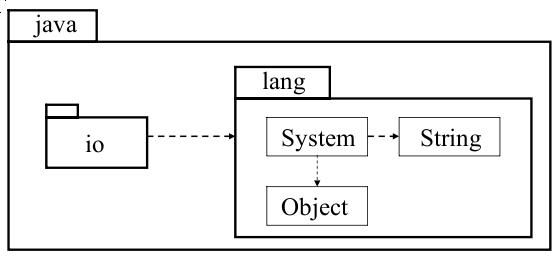
\includegraphics[width=0.6\textwidth]{fig01.png}
\end{figure}
\end{frame}

\begin{frame}
\frametitle{JDK API中的常用包}

\begin{table}
\footnotesize
\setlength{\extrarowheight}{1.2mm}
\rowcolors[]{1}{blue!20}{blue!10}
\begin{tabular}{c|p{5cm}|p{3cm}}
{\bf 包名} & {\bf 功能说明} & {\bf 包的含义}   \\
java.lang & Java语言程序设计的基础类 & language的简写\\
java.awt & 创建图形用户界面和绘制图形图像的相关类 & 抽象窗口工具集\\
java.util & 集合、日期、国际化、各种实用工具 & utility的简写\\
java.io & 可提供数据输入/输出相关功能的类 & input/output的简写\\
java.net & Java网络编程的相关功能类 & 网络\\
java.sql & 提供数据库操作的相关功能类 & 结构化查询语言的简写\\
\end{tabular}
\end{table}
\end{frame}

\begin{frame}[fragile] % [fragile]参数使得能够插入代码
\frametitle{包的创建}

package语句作为Java源文件的第一条语句,指明该文件中定义的类所在的包(若缺省该语句,则指定
为无名包)。语法格式如下:
\begin{javaCode}
package pkg1[.pkg2[.pkg3...]];
\end{javaCode}
\samp{创建包}
\begin{javaCode}
package p1;
public class Test{
  public void m1(){
    System.out.println("In class Test, 
    method m1 is running!");
  }
}
\end{javaCode}
package语句对所在源文件中定义的所有类型(包括接口、枚举、注解)均起作用。
\end{frame}

\begin{frame}[fragile] % [fragile]参数使得能够插入代码
\frametitle{包的创建}
Java编译器把包对应于文件系统的目录管理,package语句中,用“.”来指明包(目录)
的层次。如果在程序Test.java中已定义了包p1,编译时采用如下方式:
\begin{shCode}
  > javac Test.java
\end{shCode}
则编译器会在当前目录下生成Test.class文件。

若在命令行下使用如下命令:
\begin{shCode}
  > java -d /home/xiaodong/work01 Test.java
\end{shCode}
“-d /home/xiaodong/work01”是传给Java编译器的参数,用于指定此次编译生成的.class文件保存到
该指定路径下,并且如果源文件中有package语句,则编译时会自动在目标路径下创建与包同名的目
录p1,再将生成的Test.class文件保存到该目录下。
\end{frame}

\begin{frame}[fragile] % [fragile]参数使得能够插入代码
\frametitle{导入包中的类}

为使用定义在不同包中的Java类,需用import语句来引入所需要的类。语法格式:
\begin{javaCode}
import pkg1[.pkg2...].(classname|*);  
\end{javaCode}

\samp{导入和使用有名包中的类}
\begin{javaCode}
  import p1.Test; //or import p1.*;
  public class TestPackage{
    public static void main(String args[]){
      Test t = new Test();
      t.m1();
    }
  }
\end{javaCode}

\end{frame}

\begin{frame}[fragile] % [fragile]参数使得能够插入代码
\frametitle{Java包特性}

{\hei 一个类如果未声明为public的,则只能在其所在包中被使用},其他包中的类即使在源文件中使
用import语句也无法引入它。可以不在源文件开头使用import语句导入要使用的有名包中的类,而是
在程序代码中每次用到该类时都给出其完整的包层次,例如:
\begin{javaCode}
  public class TestPackage{ 
    public static void main(String args[]){ 
      p1.Test t = new p1.Test(); 
      t.m1(); 
    } 
  }
\end{javaCode}
\end{frame}

\section{继承}

\begin{frame}[fragile] % [fragile]参数使得能够插入代码
\frametitle{什么是继承?}

继承(Inheritance)是面向对象编程的核心机制之一,其本质是在已有类型基础之上进行扩充或改
造,得到新的数据类型,以满足新的需要。

根据需要定义Java类描述“人”和“学生”信息:
\samp{Class Person}
\begin{javaCode}
  public class Person {
    public String name;
    public int age;
    public Date birthDate;
    public String getInfo() {...}
  }
\end{javaCode}
\end{frame}

\begin{frame}[fragile] % [fragile]参数使得能够插入代码
\frametitle{什么是继承}

\samp{Class Student}
\begin{javaCode}
  public class Student {
    public String name;
    public int age;
    public Date birthDate;
    public String school;
    public String getInfo() {...}
  }
\end{javaCode}

通过继承,简化Student类的定义:
\samp{Class Student extends Person}
\begin{javaCode}
  public class Student extends Person {
    public String school;
  }
\end{javaCode}
\end{frame}

\begin{frame}[fragile] % [fragile]参数使得能够插入代码
\frametitle{继承}

Java类(继承其他类)声明语法格式:

\begin{javaCode}
  [< 修饰符 >] class < 类名 > [extends < 父类名 >] {
    [< 属性声明 >]
    [< 构造方法声明 >]
    [< 方法声明 >]
  }
\end{javaCode}

Object类是所有Java类的最高层父类,如果在类的声明中未使用extends关键字指明其父类,则默认父
类为Object类 。
\end{frame}

\begin{frame}[fragile] % [fragile]参数使得能够插入代码
\frametitle{Java继承的特性}

Java只支持单继承,不允许多重继承。

\begin{itemize}
\item 一个子类只能有一个父类;
\item 一个父类可以派生出多个子类。
\end{itemize}

\begin{figure}
\centering
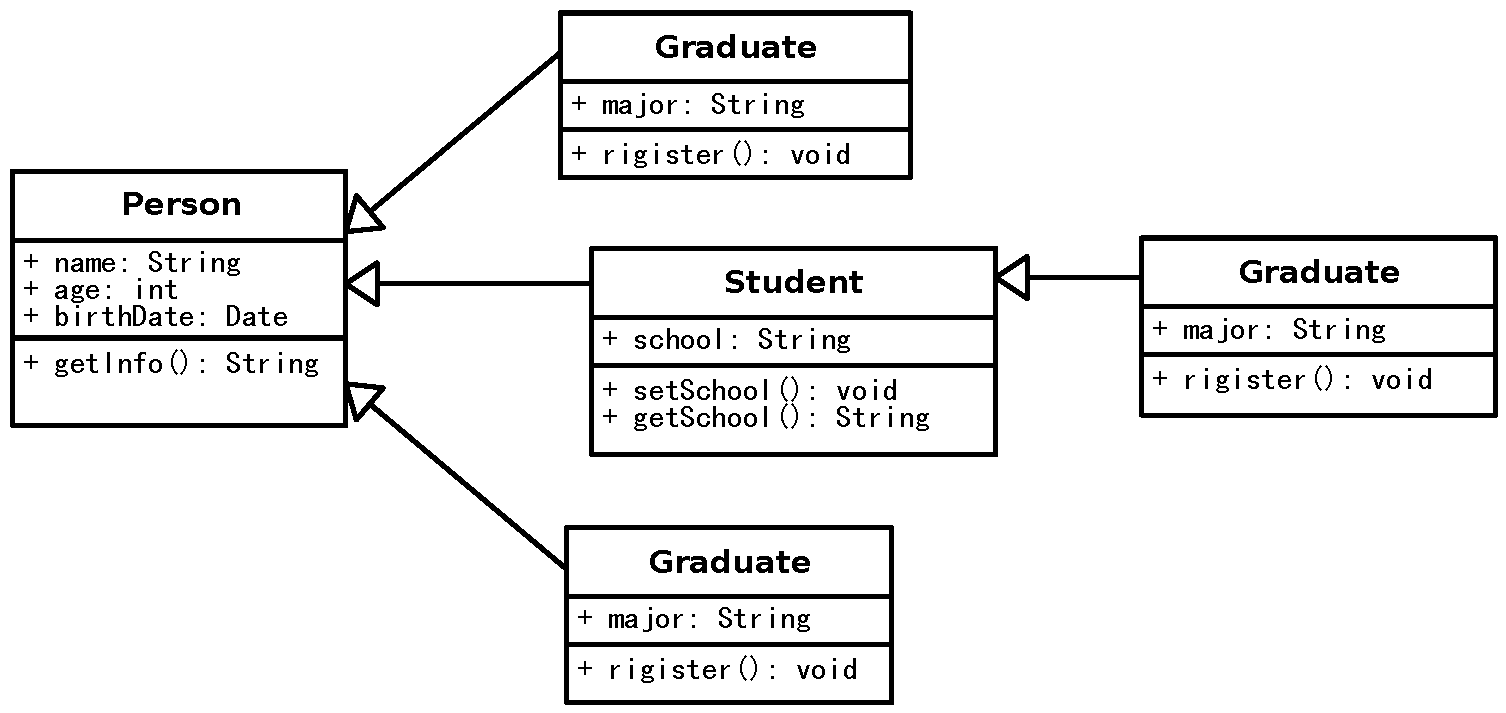
\includegraphics[width=0.7\textwidth]{a.pdf}
\end{figure}
\end{frame}



\begin{frame}[fragile] % [fragile]参数使得能够插入代码
\frametitle{类之间的关系}

\begin{description}
\item[依赖关系] 一个类的方法中使用到另一个类的对象(uses-a)\footnote{车能够装载货物,车
    的装载功能(load()方法)对货物(goods)有依赖。}。
\item[聚合关系] 一个类的对象包含(通过属性引用)了另一个类的对象(has-a)\footnote{车有发
    动机、车轮等,Car对象是由Engine等对象构成的。}。
\item[泛化关系] 一般化关系(is-a),表示类之间的继承关系、类和接口之间的实现关系以及接口
  之间的继承关系。
\end{description}
\end{frame}

\section{访问控制}
\begin{frame}[fragile] % [fragile]参数使得能够插入代码
\frametitle{访问控制}

访问控制是指对Java类或类中成员的操作进行限制,即规定其在多大的范围内可以被直接访问。
\wxd{类的访问控制}\\
在声明Java类时可以在class关键字前使用public来修饰,也可以不使用该修饰符。public的类可在任
意场合被引入和使用,而非public的类只能在其所在包中被使用。

\wxd{类中成员的访问控制}\\
\begin{table}
\footnotesize
\setlength{\extrarowheight}{1.2mm}
\rowcolors[]{1}{blue!20}{blue!10}
\begin{tabular}{c|c|c|c|c}
{\bf 修饰符/作用范围} & {\bf 同一个类} & {\bf 同一个包} & {\bf 子类} & {\bf 任何地方} \\
public & yes & yes & yes & yes\\
protected  & yes & yes & yes & no \\
无修饰符 & yes & yes & no & no \\
private & yes & no & no & no \\
\end{tabular}
\end{table}
\end{frame}

\begin{frame}[fragile] % [fragile]参数使得能够插入代码
\frametitle{访问控制}

\begin{figure}
\centering
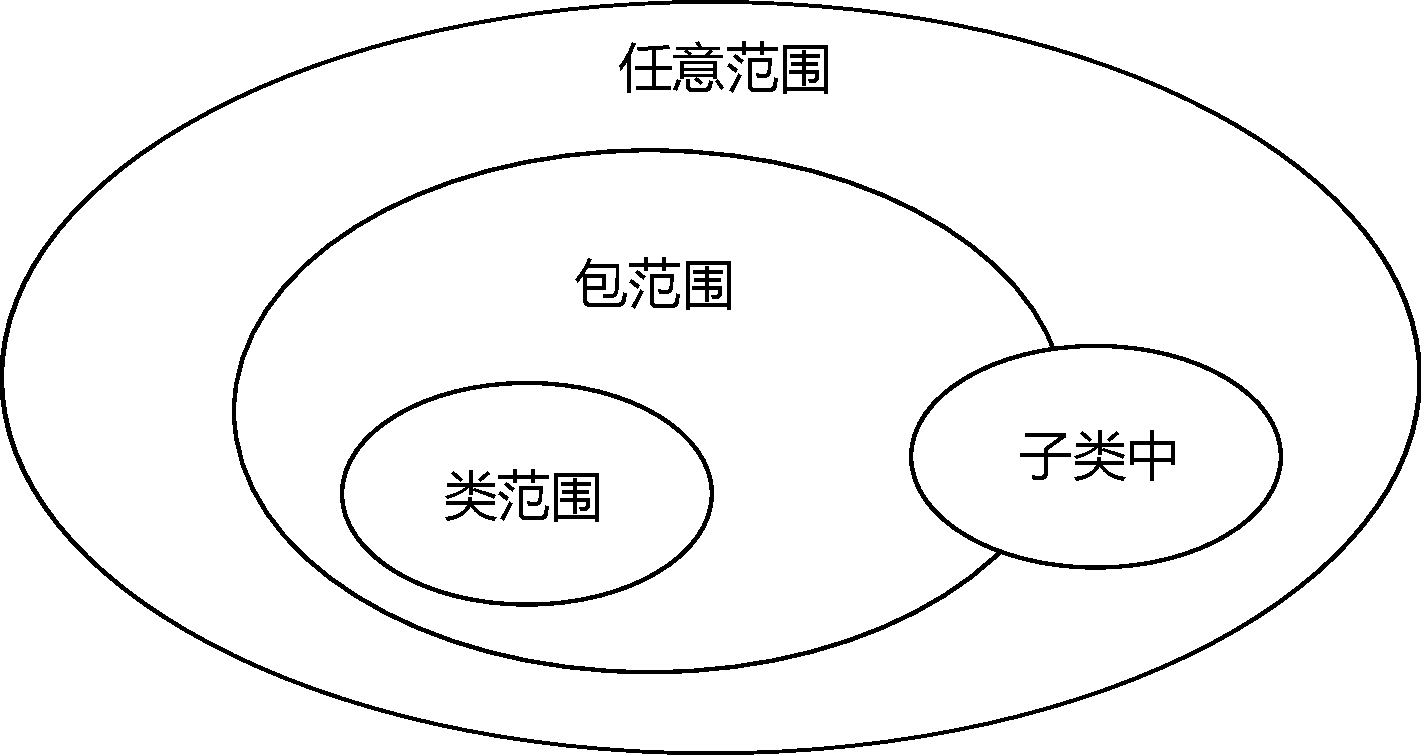
\includegraphics[width=0.7\textwidth]{fig02.pdf}
\end{figure}
\end{frame}

\begin{frame}[fragile] % [fragile]参数使得能够插入代码
\frametitle{访问控制注意的一些问题}

\begin{itemize}
\item 一般不提倡将属性声明为public的,而构造方法和需要外界直接调用的普通方法则适合声明为
  public的。
\item 在位于不同的包内,必须是子类的对象才可以直接访问其父类的protected成员,而父类自身
  的对象反而不能访问其所在类中声明的protected成员。
\item 所谓“访问控制”只是控制对Java类或类中成员的直接访问,而间接访问是不做控制的,也不该
  进行控制。
\end{itemize}

\end{frame}

\begin{frame}[fragile] % [fragile]参数使得能够插入代码
\frametitle{访问控制protected}

\samp{A.java}
\begin{javaCode}
package p1;
public class A {
  public int m = 5;
  protected int n = 6;
}
\end{javaCode}

\samp{B.java}
\begin{javaCode}
package p2;
import p1.A;
public class B extends A{
  public void mb() {
    m = m + 1;
    n = n * 2;
  }
  public static void main(String[] args) {
    B b = new B();
    b.m = 7;  // 合法
    b.n = 8;   // 合法
    A a = new A();
    a.m = 9 // 合法
    a.n = 10 // 非法
  }
}
\end{javaCode}
\end{frame}

\section{方法重写}
\begin{frame}[fragile] % [fragile]参数使得能够插入代码
\frametitle{方法重写}

\wxd{什么是方法重写}\\
在子类中可以根据需要对从父类中继承来的方法进行重新定义,此称方法重写(Override)或覆盖。

\wxd{语法规则}\\
\begin{itemize}
\item 重写方法必须和被重写方法具有相同的方法名称、参数列表和返回值类型;
\item 重写方法不能使用比被重写方法更严格的访问权限;
\item 重写方法不允许声明抛出比被重写方法范围更大的异常类型。
\end{itemize}
\end{frame}

\begin{frame}[fragile] % [fragile]参数使得能够插入代码
\frametitle{方法重写示例}
\samp{方法重写示例A}
\begin{javaCode}
public class Person {
  String name;
  int age;
  public String getInfo() {
    return "Name:"+ name + "\t" +"age:"+ age;
  }
}
\end{javaCode}

\begin{javaCode}
public class Student extends Person {
  private String school;
  public void setSchool(String scholl) {
    this.school = school;
  }
  public String getSchool(){
    return school;
  }
  public String getInfo() {
    return "Name:"+ name + "\tAge:"+ age + "\tSchool:" + school;
  }
}
\end{javaCode}
\end{frame}

\begin{frame}[fragile] % [fragile]参数使得能够插入代码
\frametitle{方法重写示例}
\samp{方法重写示例B}
\begin{javaCode}
public class Parent {
  public void method1() {...}
}
\end{javaCode}

\begin{javaCode}
public class Child extends Parent {
  private void method1() {} //非法,权限更严格
}
\end{javaCode}

\begin{javaCode}
public class UseBoth {
  public void doOtherThing() {
    Parent p1 = new Parent();
    Child p2 = new Child();
    p1.method1();
    p2.method1();
  }
}
\end{javaCode}
\end{frame}

\begin{frame}[fragile] % [fragile]参数使得能够插入代码
\frametitle{同名属性}
\samp{同名属性}
\begin{javaCode}
  public class Person {
    int age = 5;
    public int getAge() {
      return age;
    }
    public int getInfo() {
      return age;
    }
  }
  \end{javaCode}

  \begin{javaCode}
  public class Student extends Person {
    int age = 6;
    public int getAge() {
      return age;
    }
  }
\end{javaCode}
\end{frame}

\begin{frame}[fragile] % [fragile]参数使得能够插入代码
\frametitle{同名属性}
\begin{javaCode}
  public class Test {
    public static void main(String args[]) {
      Person p = new Person();
      System.out.println(p.getAge());
      Student s = new Student();
      System.out.println(s.age);
      System.out.println(s.getAge());
      System.out.println(s.getInfo());
    }
  }
\end{javaCode}

输出结果:
\begin{stdoutCode}
5
6
6
5
\end{stdoutCode}
\end{frame}

\begin{frame}
\frametitle{同名属性}
\wxd{对上述Student对象同名属性的几点说明}  
\begin{enumerate}
\item 以“对象名.属性名”方式直接访问时,使用的是子类中添加的属性age;
\item 调用子类添加或者重写的方法时,方法中使用的是子类定义的属性age;
\item 调用父类中定义的方法时,方法中使用的是父类中的属性age。
\end{enumerate}
{\hei 可以理解为“层次优先”\footnote{在哪个层次中的代码,就优先使用该层次类中定义的属性。};\Red 不提倡使用同名属性。}
\end{frame}

\section{关键字super} 
\begin{frame}[fragile] % [fragile]参数使得能够插入代码
\frametitle{关键字super}

在存在命名冲突(子类中存在方法重写或添加同名属性)的情况下,子类中的代码将自动使用子类中
的同名属性或重写后的方法。当然也可以在子类中{\Red 使用关键字super引用父类中的成分}:

\xyy{访问父类中定义的属性}\\
super.<属性名>
\xyy{调用父类中定义的成员方法}\\
super.<方法名>(<实参列表>)
\xyy{子类构造方法中调用父类的构造方法}\\
super(<实参列表>)

super的追溯不仅限于直接父类,先从直接父类开始查找,如果找不到则逐层上溯,一旦在某个层次父
类中找到匹配成员即停止追溯并使用该成员。
\end{frame}

\begin{frame}[fragile] % [fragile]参数使得能够插入代码
\frametitle{super用法示例}

\samp{super A}
\begin{javaCode}
  class Animal {
    protected int i = 1;   //用于测试同名属性,无现实含义
  }

  class Person extends Animal {
    protected int i = 2;     //用于测试同名属性,无现实含义
    private String name = "Tom";
    private int age = 9;
    public String getInfo() {
      return "Name:" + name + "\tAge:" + age;
    }
    public void testI() {
      System.out.println(super.i);
      System.out.println(i);
    }
  }
  
\end{javaCode}
\end{frame}

\begin{frame}[fragile] % [fragile]参数使得能够插入代码
\frametitle{super用法示例}

\samp{super B}
\begin{javaCode}
  class Student extends Person {
    private int i = 3;
    private String school = "THU";
    public String getInfo() {       //重写方法
      return super.getInfo() + "\tSchool:" + school;
    }
    public void testI() {       //重写方法
      System.out.println(super.i);
      System.out.println(i);
    }
  }
  public class Test {
    public static void main(String args[]) {
      Person p = new Person();
      System.out.println(p.getInfo());
      p.testI();
      Student s = new Student();
      System.out.println(s.getInfo());
      s.testI();
    }
  }
\end{javaCode}
\end{frame}

\begin{frame}[fragile] % [fragile]参数使得能够插入代码
\frametitle{super用法示例}

上述代码的输出结果:
\begin{stdoutCode}
Name:Tom Age:9
1
2
Name:Tom Age:9 School:THU
2
3  
\end{stdoutCode}
\end{frame}



\section{关键字this}
\begin{frame}[fragile] % [fragile]参数使得能够插入代码
\frametitle{关键字this}
在Java方法中,不但可以直接使用方法的局部变量,也可以使用调用该方法的对象。

为解决可能出现的命名冲突,Java语言引入this关键字来标明方法的当前对象。分为两种情况:
\begin{itemize}\kai
\item 在普通方法中,关键字this代表方法的调用者,即本次调用了该方法的对象;
\item 在构造方法中,关键字this代表该方法本次运行所创建的那个新对象。
\end{itemize}
this作为一个特殊的引用类型变量,可以通过“{\Red this.成员}”的方式访问其引用的当前对象的属性和方法。
\end{frame}

\begin{frame}[fragile] % [fragile]参数使得能够插入代码
\frametitle{关键字this}
\samp{this用法示例}
\begin{javaCode}
public class MyDate {
  private int day = 17;
  private int month = 2;

  public MyDate(int day, int month) {
    this.day = day; // A
    this.month = month;
  }
  ... // Some methods 

  public void setAll(int day, int month) {
    this.setMonth(month); // B
    this.setDay(day);
  }
}
\end{javaCode}
\end{frame}

\begin{frame}[fragile] % [fragile]参数使得能够插入代码
\frametitle{关键字this}

\wxd{关于this的归纳说明}
\begin{enumerate}
\item 在Java方法中直接给出变量名而不是“对象名.变量名”的方式访问一个变量,系统首先尝试作为
  局部变量来处理;如果方法中不存在该名字的局部变量,才会到方法当前对象的成员变量中查找。
\item 在Java方法中直接调用一个方法而不指定其调用者时,则默认调用者为当前对象this。
\end{enumerate}
\end{frame}

\begin{frame}[fragile] % [fragile]参数使得能够插入代码
  \frametitle{本节习题}

  \begin{enumerate}
  \item 类之间具备哪些关系?
  \item 比较说明super和this的含义。
  \end{enumerate}
\end{frame}

%%%%%%%%%%%%%%%%%%%%%%%%%%%%%%%%%%%%%%%%%%%%%%%%%%%%%%%%%%%%%%%%%%%%%%%%%%%%%%%
% TKS Page %%%%%%%%%%%%%%%%%%%%%%%%%%%%%%%%%%%%%%%%%%%%
\begin{frame}
\centering
{\Huge \textcolor{blue}{THE END}} \\
\vspace{5mm}
{\Large wangxiaodong@ouc.edu.cn} \\
\end{frame}
%%%%%%%%%%%%%%%%%%%%%%%%%%%%%%%%%%%%%%%%%%%%%%%%%%%%%%%
%%%%%%%%%%%%%%%%%%%%%%%%%%%%%%%%%%%%%%%%%%%%%%%%%%%%%%%%%%%%%%%%%%%%%%%%%%%%%%%
\end{document}
